\section{Proposed Approach}
\label{sec:approach}
% \jh{Comment 1: Need to explain PatchNet in a good way so that non-expert ML can understood (reviewer A) -- Need to rewrite the section~\ref{sec:approach}}

In this section, we first formulate the problem and provide an overview of PatchNet. We then describe the details of each module inside PatchNet. Finally, we present an algorithm for learning effective settings of PatchNet's parameters.
% Finally, we present the algorithms for learning model parameters.

\vspace{-0.5em}
\subsection{Framework Overview}
\label{sec:overall_framework}

The goal of PatchNet is to automatically label a
patch as stable or non-stable in order to reduce the manual effort for the stable-kernel maintainers. 
% Let $\mathcal{X} = \{x_1, \dots, x_N \}$ denote
% the set of patches that have been accepted into the mainline kernel, where
% $N$ is the number of patches considered.
% \jl{Do we ever use $N$? If not, drop this explanation.} \jl{I put this
%   question back because I still don't see where we use $N$}.
We consider the identification of stable patches as a learning task to construct a prediction function $f:
\mathcal{X} \longmapsto \mathcal{Y}$, where $\mathcal{Y} = \{0, 1\}$. In
this case, $x_i \in \mathcal{X}$ is identified as a stable patch when $f(x_i) = 1$, and 0 otherwise.
% $y_i \in \mathcal{Y}$ 
% \jl{Why say $y_i$ instead of $f(x_i)?$}
% \jg{$y_i$ is the true label and $f(x_i)?$ is the predicted label}
% \jl{It doesn't say that anywhere at all.}
% is 1 when patch $x_i \in \mathcal{X}$ is identified as a
% stable patch, and 0 otherwise.

As illustrated in Figure~\ref{fig:patchnet}, PatchNet consists of three
main modules: (1) a \textit{commit message module}, (2) a \textit{commit
  code module}, and (3) a \textit{classification module}.  The first two
are built upon a CNN-based architecture~\cite{lecun1998gradient, krizhevsky2012imagenet}, and aim
to learn a representation of the textual commit message
(cf. Figure~\ref{fig:sample_patch}, lines 5-12) and the set of diff code
elements (cf. Figure~\ref{fig:sample_patch}, lines 14-28) of a patch,
respectively.  The \textit{commit message module} and the \textit{commit
  code module} transform the commit message and the code changes into
embedding vectors $\mathbf{e}_m$ and $\mathbf{e}_c$, respectively. The two
vectors are then passed to the \textit{classification module}, which aims to compute a prediction score indicating the likelihood of a patch being a stable patch.
% \ty{pls verify}

\begin{figure}[!t]
	\center
	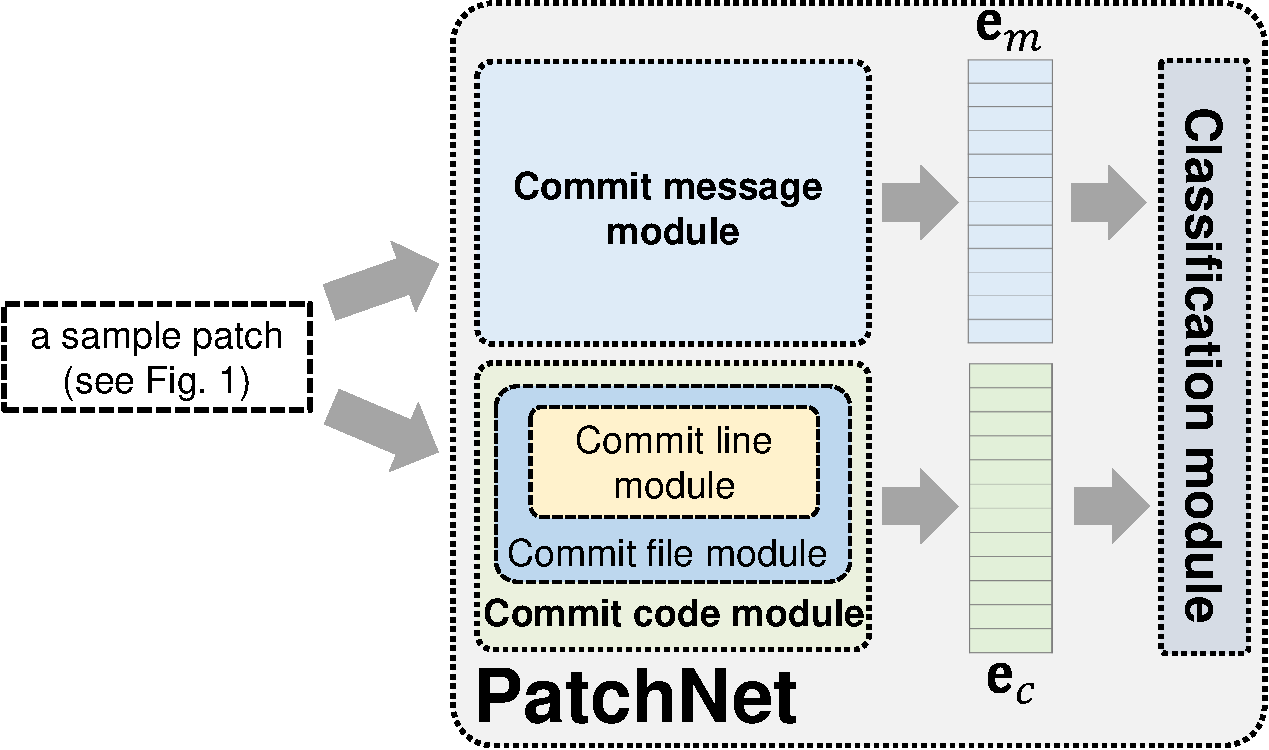
\includegraphics[scale=0.37]{figures/framework_overall_ver1.pdf}
	\caption{The proposed PatchNet framework. $\textbf{e}_m$ and $\textbf{e}_c$ are embedding vectors collected from the commit message module and commit code module respectively.}
	\label{fig:patchnet}
    \vspace{-0.4cm}
\end{figure}

\subsection{Commit Message Module}
\label{sec:commit_msg_model}

%The design of our \textit{commit message module} is built on the work of Kim~\cite{kim2014convolutional} and Kalchbrenner {\em et al.}~\cite{kalchbrenner2014convolutional} on sentence classification. 

%Figure~\ref{fig:msg_model} shows the architecture of the commit message module. The module uses CNN and involves an input message, represented as a two-dimensional matrix, a set of filters for identifying features in the message, and a means of combining the results of the filters into an \textit{embedding vector} that represents the most salient features of the message, to be used as a basis for classification.

Figure~\ref{fig:msg_model} shows the architecture
of the commit message module, which is the same as the one proposed by Kim~\cite{kim2014convolutional} for sentence classification. This module takes a commit message as input and outputs an embedding vector that represents the most salient features of the message.


\begin{figure}
\center
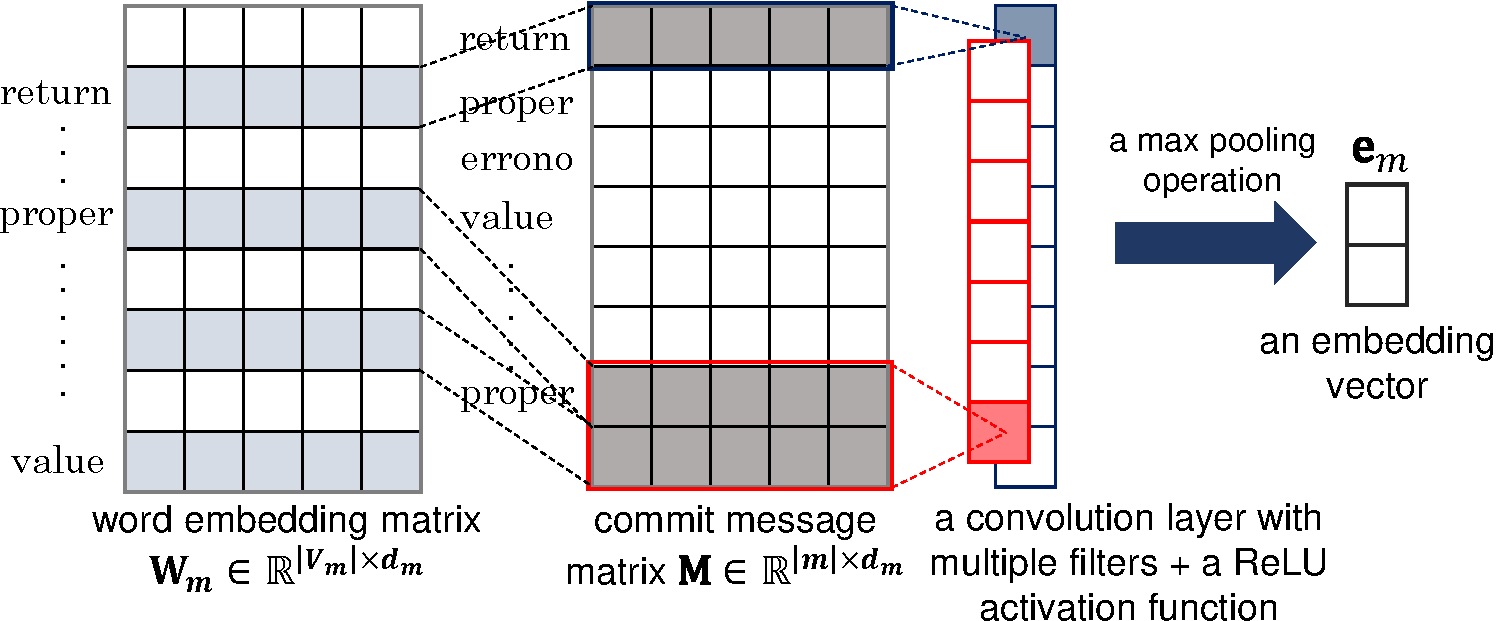
\includegraphics[scale=0.36]{figures/msg_model_ver2.pdf}
\caption{Architecture of our \textit{commit message module} used to build an embedding vector from a commit message.}
\label{fig:msg_model}
\vspace{-0.4cm}
\end{figure}

% \jl{Figure \ref{fig:msg_model} should have only two entries in the
%   embedding vector.}

\textbf{Message representation}. We encode a commit message as a
two-dimensional matrix by viewing the message as a sequence of vectors
where each vector represents one word appearing in the
message. The embedding vectors of the individual words are maintained using a
lookup table, the {\em word embedding matrix}, that is shared across all
messages.

Given a message $m$ as a sequence of words
$[\texttt{w}_1, \dots, \texttt{w}_{|m|}]$ and a word embedding matrix
$\textbf{W}_m \in \mathbb{R}^{|V_m|\times d_m}$, where $V_m$ is the vocabulary containing all words in commit messages and  $d_m$ is the
dimension the representation of a word, the matrix representation
$\textbf{M} \in \mathbb{R}^{|m| \times d_m}$ of the message is:
\begin{equation} \footnotesize
\textbf{M} =
[\textbf{W}[\texttt{w}_1], \dots, \textbf{W}[\texttt{w}_{|m|}]]
\end{equation}
For parallelization, all messages are padded or truncated to same length.

\textbf{Convolutional layer}. The role of the convolutional layer is to apply
filters to the message, in order to identify the message's salient
features.  
% \jl{convolution or convolutional?} \jg{It's the convolutional layer, more details can be found \href{https://en.wikipedia.org/wiki/Convolutional_neural_network}{here}}
%In our setting \jl{Can we drop ``In our setting''?}, 
A filter $\textbf{f} \in \mathbb{R}^{k \times d_m}$ is
a small matrix 
% \ty{actually, i feel it is product of f and M, not element-wise product...btw, f looks like a function, but it is a weight matrix, a little bit confusing here.} 
that is applied
to a window of $k$ words to produce a new feature. A feature $t_i$ is generated from a window of words
$\textbf{M}_{i:i+k-1}$ starting at word $i \leq |m|- k + 1$ by:
% \jl{$i \leq |m|- k+1$???}
\begin{equation} \footnotesize
\label{eq:filtering}
t_i = \alpha ( \textbf{f} \ast \textbf{M}_{i:i+k-1} + b_i) 
\end{equation}
where $\ast$ is a sum of element-wise products, $b_i \in
\mathbb{R}$ is a bias value, and $\alpha(\cdot)$ is a non-linear activation
function. For $\alpha(\cdot)$, we choose the rectified linear unit (ReLU) activation function~\cite{nair2010rectified}, as it has been shown to have better performance than 
its alternatives~\cite{anastassiou2011univariate,dahl2013improving}.
% logistic sigmoid and hyperbolic tangent~\cite{anastassiou2011univariate,dahl2013improving}.
%\jl{not grammatical, and I don't know what is meant}\ty{modified}
% significant benefits in terms of \jl{could we drop ``significant benefits
% in terms of''? It seems like a lot of words for no meaning.} 
%faster training, sparse activation, and
%reduced likelihood of vanishing %gradients~\cite{han1995influence,anastassiou2011univariate,dahl2013improving}. 
The filter $\textbf{f}$ is applied to all windows of size $k$ in the message resulting in a \textit{feature vector} $\textbf{t} \in \mathbb{R}^{|m|-k+1}$:
\begin{equation} \footnotesize
\label{eq:ftr_vector}
\textbf{t} = [t_1, t_2, \cdots, t_{|m|-k+1}]
\end{equation}


\textbf{Max pooling}. 
To characterize the commit message, we are interested in the degree to
which it contains various features, but not where in the message those
features occur. Accordingly, for each filter,
% To capture the most important feature in each feature vector, 
we apply a max pooling operation~\cite{collobert2011natural} over the feature vector $\textbf{t}$ to obtain the highest value:
% and take the maximum value as the feature corresponding to a particular filter:
\begin{equation} \footnotesize
\label{eq:pooling}
\underset{1 \leq i \leq |m|-k+1}{\max} t_i
\end{equation}

\noindent
The results of applying max pooling to the feature vector resulting from
applying each filter are then concatenated to form an embedding vector
($\mathbf{e}_m$ on the right side of Figure~\ref{fig:msg_model})
representing the meaning of the message.
% \jg{Look at David's comment}

\subsection{Commit Code Module}
\label{sec:commit_code_model}
Like the commit message,
the commit code can be viewed as a sequence of words. This view, however, overlooks the structure of code changes, as needed to distinguish between changes to different files, changes in
different hunks, and different kinds of changes (removals or additions). To incorporate this structural information, PatchNet contains a {\em Commit Code Module} that takes as input the code changes in a given patch and outputs an embedding vector that represents the most salient features of the code changes. The Commit Code Module contains a {\em Commit File Module} that automatically builds an embedding vector representing the code changes made to a given file in the patch. The embedding vectors of code changes at file level are then concatenated into a single vector representing all the code changes made by the patch.

\subsubsection{Commit file module}
\label{sec:code_file_framework}

The goal of the commit file module is to build an embedding vector
for each file in the patch that represents the changes that affect the file.

As shown in Figure~\ref{fig:commit_code_model}, the commit file module
takes as input two matrices (denoted by ``--'' and ``+'' in
Figure~\ref{fig:commit_code_model}) representing the removed code and added
code for the affected file in a patch, respectively. These two matrices
are passed to the \textit{removed code module} and the \textit{added code
module}, respectively, to construct corresponding embedding vectors. The two embedding vectors are then concatenated to represent the code changes in each affected file. We present the removed code module and the added code module below.

\begin{figure}[t!]
	\center
	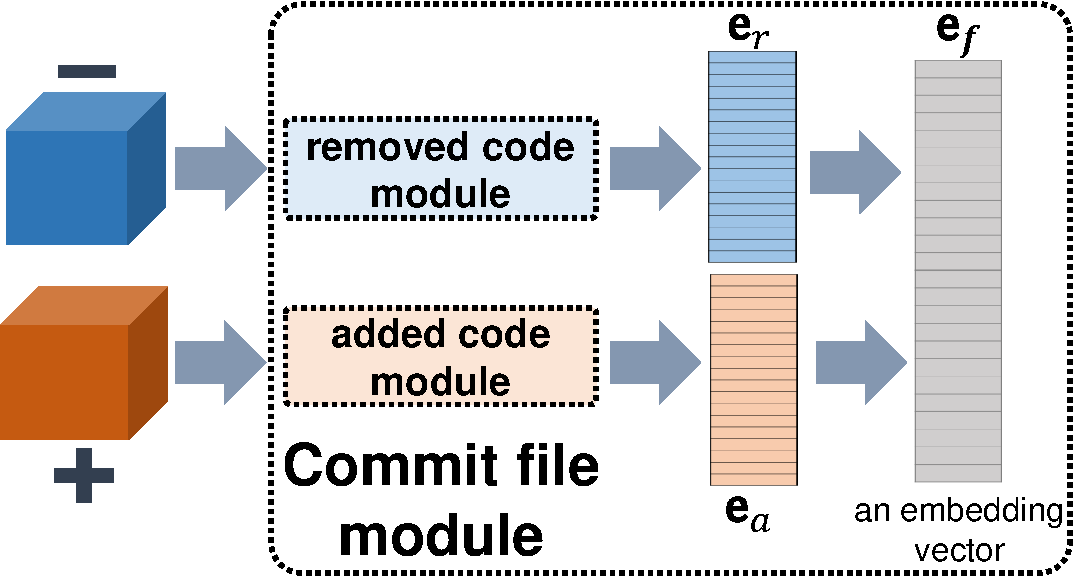
\includegraphics[scale=0.43]{figures/commit_file_model.pdf}
	\caption{Architecture of the \textit{commit file module} for
          mapping a file in a given patch to an embedding vector. The input
          of the module is the removed code and added code of the affected
          file, denoted by ``--'' and ``+'', respectively.}
	\label{fig:commit_code_model}
\end{figure}

\textbf{\textit{Removed code module.}} Figure~\ref{fig:cnn3d}
shows the structure of the \textit{removed code module}. The
input of this module is a three-dimensional matrix, indicating the removed code
in a file of a given patch, denoted by $\mathcal{B}_r \in
\mathbb{R}^{\mathcal{H} \times \mathcal{N} \times \mathcal{L}}$, where
$\mathcal{H}$, $\mathcal{N}$, and $\mathcal{L}$ are the number of hunks,
the number of removed code lines for each hunk, and the number of words of each
removed code line in the affected file, respectively. This module
constructs an embedding vector (denoted by $\textbf{e}_r$ in Figure~\ref{fig:commit_code_model}) representing the removed code in the affected file.

\begin{figure*}[t!]
	\center
	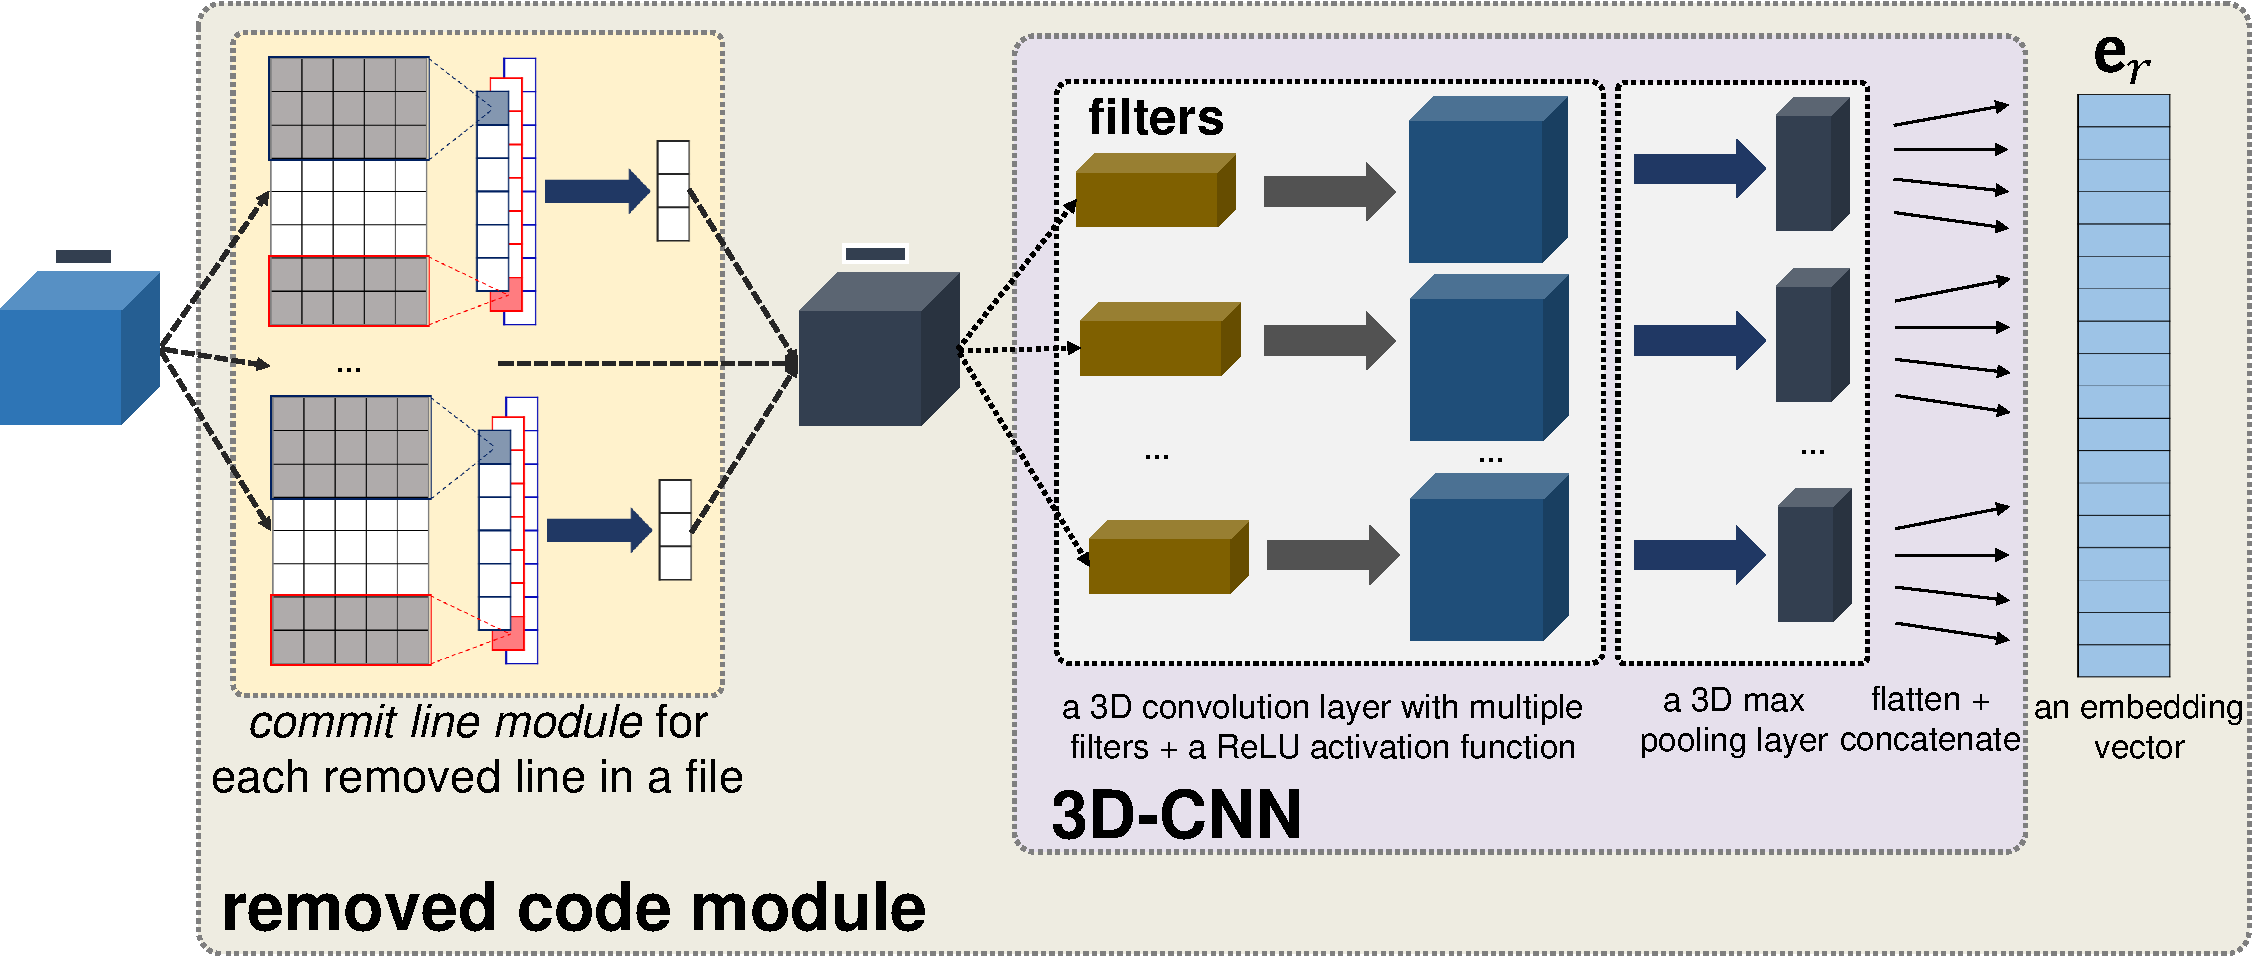
\includegraphics[scale=0.38]{figures/cnn-3d_ver1.pdf}
	\caption{Architecture of the \textit{removed code module} used to build an embedding vector for the code removed from an affected file.}
	\label{fig:cnn3d}
\end{figure*}

\textit{a) Commit line module.}  Each line of removed code in
$\mathcal{B}_r$ is processed by the {\em commit line module} to obtain a
list of embedding vectors representing the removed code lines. This module
has the same structure as the commit message module, but maintains a
code-specific vocabulary and word embedding matrix, as a word may have
different meanings in a textual message and in source code.

The obtained commit line vectors are used to construct a new three-dimensional matrix,
$\hat{\mathcal{B}}_r \in \mathbb{R}^{\mathcal{H} \times \mathcal{N} \times
  E}$. $\hat{\mathcal{B}}_r$ represents a sequence of ${\mathcal{H}}$
hunks; each hunk has a sequence of removed lines, where each line is now
represented as a $E$-dimensional embedding vector ($e_{ij} \in \mathbb{R}^E$) extracted by
the \textit{commit line module}. $\hat{\mathcal{B}}_r$ is then passed to the
3D convolutional neural network (3D-CNN), described below, to construct an embedding vector for the code removed from a file by a given patch.

\textit{b) 3D-CNN}.
% \ty{this is a module or a layer? it contains multiple layers right?} \jg{It's a filter}
The 3D convolutional layer is used to
extract features from the code removed from the affected file, as
represented by $\hat{\mathcal{B}}_r$.  This layer applies each
filter $\textbf{F} \in \mathbb{R}^{k \times \mathcal{N} \times E}$
to a window of $k$ hunks $\textbf{H}_{i:i+k-1}$ to build a new feature as
follows:
\begin{equation} \footnotesize
\label{eq:3d_filter}
f_i = \alpha(\textbf{F} \ast \textbf{H}_{i:i+k-1} + b_i) ]
\end{equation}
% \ty{make sure its element-wise or dots}
$\ast$ is the sum of element-wise products, $\textbf{H}_{i:i+k-1} \in
\mathbb{R}^{|i:i+k-1| \times\mathcal{N} \times E}$ is constructed from the
$i$-th hunk through the $(i+k-1)$-th hunk in the removed code of the affected
file, $b_i \in \mathbb{R}$ is the bias value, and $\alpha(\cdot)$ is the
ReLU activation function. As in Section~\ref{sec:commit_msg_model}, we
choose $k \in \{1, 2\}$. 
% Figure~\ref{fig:filtering_example} shows an example of a 3D convolutional layer that has one filter.
%\begin{figure}[t!]
%	\center
%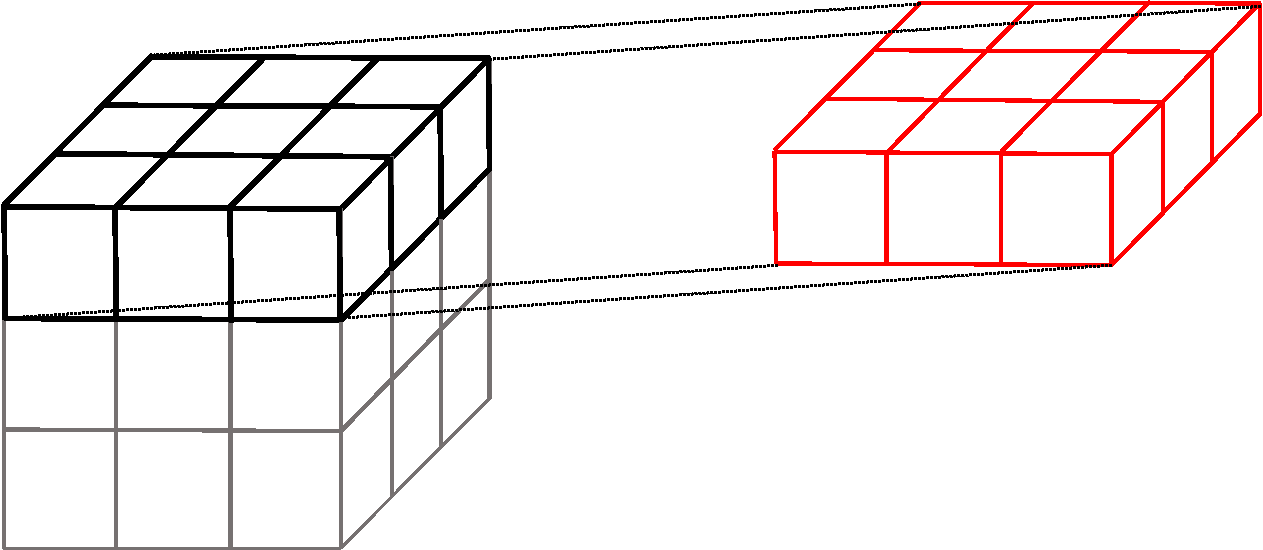
\includegraphics[scale=0.25]{figures/filtering_example.pdf}
%	\caption{A 3D convolutional layer on $3 \times 3 \times 3$ data. The $1 \times 3 \times 3$ red cube on the right is the filter. The dotted lines indicate the sum of element-wise products over all three dimensions. The result is a scalar in every instance of the operation.}
%	\label{fig:filtering_example}
%    \vspace{-0.4cm}
%\end{figure}
Applying the filter $\textbf{F}$ to all windows of hunks in
$\hat{\mathcal{B}_r}$ produces a feature vector: 
\begin{equation} \footnotesize
\label{eq:ftr_hunk}
\mathcal{F} = [f_1, \dots, f_{\mathcal{H} - k + 1}]
\end{equation}

As in Section~\ref{sec:commit_msg_model}, we apply a max pooling operation
to $\mathcal{F}$ to obtain the most important feature.
% , {\em i.e.}, the most important hunks representing information about the removed code changes. 
The features selected by max pooling with multiple filters are concatenated to
construct an embedding vector $\textbf{e}_r$ representing information
extracted from the removed code changes in the affected file.
%of a given patch. 
%(see the last layer in Figure~\ref{fig:cnn3d}).

\textbf{\textit{Added code module}} The \textit{added code module} follows
the same architecture as the removed code module. These changes in the
added and removed code are furthermore padded or truncated to have the same
number of hunks ($\mathcal{H}$), number of lines for each hunk
($\mathcal{N}$), and the number of words of each line ($\mathcal{L}$) for
parallelization. Moreover, both modules also share the same vocabulary and
use the same word embedding matrix.

The added code module
constructs an embedding vector (denoted by $\textbf{e}_a$ in Figure~\ref{fig:commit_code_model}) representing the added code in a file
of a given patch. An embedding vector representing all of the changes made to a given file by a commit is constructed by
concatenating the two embedding vectors representing the removed code and
added code, i.e., $\textbf{e}_\texttt{f} = \textbf{e}_r \oplus \textbf{e}_a$. 

% \jg{Julia: can you please recheck these two paragraph above?}

%\begin{equation} \footnotesize
%\label{eq:commit_file}
%\textbf{e}_\texttt{f} = \textbf{e}_r \oplus \textbf{e}_a
%\end{equation}  

% For parallelization, the removed and added code are furthermore padded or truncated to be the same number of hunks, number of lines for each hunk, and number of words per line.

\subsubsection{Constructing an embedding vector for commit code}
\label{sec:construct_commit_code}
The embedding vector for all the changes performed by a given patch is constructed as follows:
\begin{equation} \footnotesize
\label{eq:commit_code_vector}
\textbf{e}_c = \textbf{e}_{\texttt{f}_1} \oplus \dots \oplus \textbf{e}_{\texttt{f}_v}
\end{equation}
where $\oplus$ is the concatenation operator, $\texttt{f}_i$ denotes the $i$-th file affected by the given commit, $v$ is the number of affected files, and $\textbf{e}_{\texttt{f}_i}$ denotes the vector constructed by applying the commit file module to the affected file $\texttt{f}_i$.


\subsection{Classification Module}
\label{sec:classification_model}

\begin{figure}[t!]
	\center
	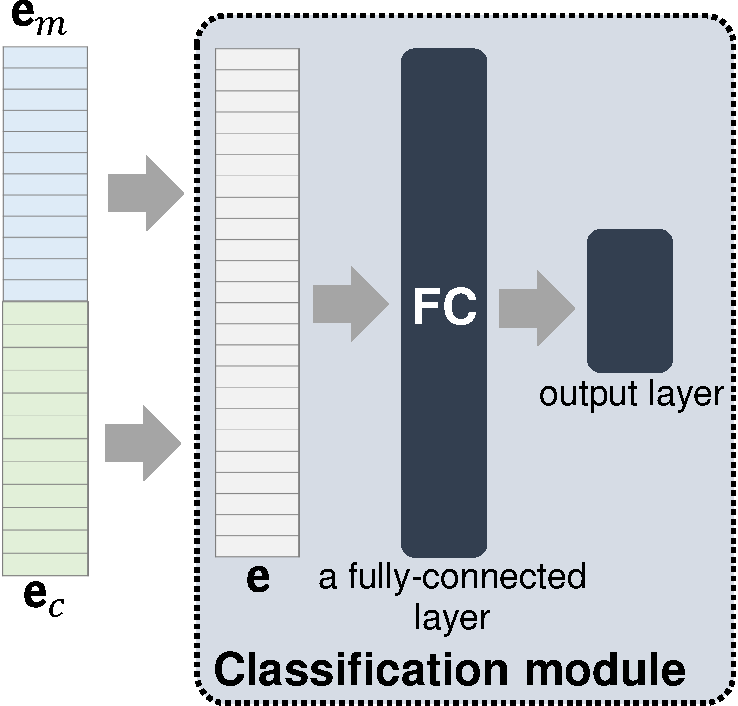
\includegraphics[scale=0.4]{figures/classification_module.pdf}
	\caption{Architecture of the \textit{classification module}, comprising a fully connected layer (FC), and an output layer.}
	\label{fig:clf_module}
    \vspace{-0.4cm}
\end{figure}

% \jl{Figure \ref{fig:clf_module} mentions a concatenation operator, but we
%   don't see it}

Figure~\ref{fig:clf_module} shows the architecture of the \textit{classification module}. It takes as input the commit message embedding vector $\mathbf{e}_m$ and the commit code embedding vector $\mathbf{e}_c$ discussed in Sections~\ref{sec:commit_msg_model} and~\ref{sec:commit_code_model}, respectively.
These two vectors are then concatenated to form a single vector representing a patch,
{\em i.e.}, $\textbf{e} = \mathbf{e}_m \oplus \mathbf{e}_c$.

We then feed the concatenated vector $\mathbf{e}$ into a fully-connected
(FC) layer, which outputs a vector
% representation \jl{what is it?} 
$\mathbf{h}$ as follows:
\begin{equation}  \footnotesize
\label{eq:fully_layer}
\mathbf{h} = \alpha(\mathbf{w}_h \cdot \mathbf{e} + b_h)
\end{equation}
where $\cdot$ is a dot product, 
% $\textbf{w}_h$ is the weight vector of the FC layer, 
$\textbf{w}_h$ is a weight matrix of the vector $\mathbf{e}$ and the FC layer and is learned during a training process,  
$b_h$ is the bias value, and $\alpha(\cdot)$ is a non-linear
activation function. Again, we use ReLU to realize $\alpha(\cdot)$.

Finally, the vector $\mathbf{h}$ is passed to an output layer, which
computes a probability score for a given patch:
\begin{equation}  \footnotesize
z_i = p(y_i=1|x_i) = \frac{1}{1 + \exp({-\mathbf{h} \cdot \mathbf{w}_o)}}
\end{equation}
% where $\mathbf{w}_o$ is the 
% weight vector of the output layer.
where $\mathbf{w}_o$ is a weight matrix 
% between the FC layer and the output layer, $\mathbf{w}_o$ 
that is also learned during our training process. 

% \jl{There is $\mathbf{\theta}$ here and $\mathbf{\theta}$ in the next
%   section, but I have no idea whether they are representing the same things.} \jg{No, they don't.}

\subsection{Parameter Learning}
\label{sec:learning}

During the training process, PatchNet learns the following parameters: the
word embedding matrices for commit messages and commit code, the filter matrices and bias of the convolutional layers, and the weights and bias of
the fully connected layer and the output layer. Training minimizes the
following standard regularized loss function~\cite{haykin2001kalman}:
\begin{equation} \footnotesize
\label{eq:cost}
\begin{split}
\mathcal{O} &= -\log\left( \prod_{i=1}^{N} p(y_i|x_i) \right) + \frac{\lambda}{2} \|\theta\|_{2}^{2} \\
 &= -\sum_{i=1}^{N} \left[ y_i \log (z_i) + (1 - y_i) \log(1 - z_i) \right] + \frac{\lambda}{2} \|\theta\|_{2}^{2}
\end{split}
\end{equation}
where $z_i$ is the probability score from the output layer and $\theta$
contains all parameters our model. 
% optimized by the network:
% \begin{align*}
% \label{eq:parameters}
% \theta = \{\textbf{W}_m, \textbf{f}, \textbf{b}, \textbf{w}_h, \text{w}_o \}
% \end{align*}
% namely the word embeddings matrix 

The term $\frac{\lambda}{2} \|\theta\|_{2}^{2}$ is used to mitigate data overfitting by penalizing large model parameters, thus reducing the model complexity. 
%Data overfitting is a common issue for neural networks, especially when the data size is small~\cite{caruana2001overfitting}. 
%To mitigate data ovefitting, 
To further improve the robustness of our model, we also apply the dropout technique~\cite{srivastava2014dropout} on the convolutional and fully-connected layers in PatchNet. 
% we add an $l_2$ regularization term \jl{It is not clear what this is.  A
%   term like the one shown here seems to be already in the above formula.
%   So it is not clear if you are describing that or how you further modify that.}
% ($\frac{\lambda}{2} \|\theta\|_{2}^{2}$) to the loss function, which
% penalizes large model parameters, thus reducing the model complexity. 

%Dropout can be viewed as a regularization technique to prevent complex co-adaptation on training data by randomly dropping neurons (units) when training a neural network. It also constitutes an efficient way for model averaging in neural networks.

To minimize the regularized loss function in (\ref{eq:cost}), we employ a
variant of stochastic gradient descent (SGD)~\cite{bottou2010large}
called \textit{adaptive moment estimation}
(Adam)~\cite{kingma2014adam}. We choose Adam over SGD due to its computational efficiency and low memory requirements~\cite{kingma2014adam, anthimopoulos2016lung, arora2018optimization}.  
% because it has been shown to converge faster and it is less sensitive to hyperparameters~\cite{}.\ty{pls add a reference here.} 
%Adam improves the convergence speed of the conventional SGD by imposing adaptive learning rate for each parameter that is computed by keeping track of the exponentially decaying average of the past gradients. We choose Adam due to its computational efficiency and low memory requirements~\cite{kingma2014adam}.  Meanwhile, to efficiently compute the gradients in linear time (with respect to the neural network size), we use backpropagation~\cite{hagan1994training}, which is a simple implementation of the chain rule of partial derivatives.

